\newpage
\section{Architecture}
A general system consists of  \textbf{elements} and \textbf{relationships} between them. The elements are the functional units with interaction of different kinds in between (e.g. data flow, request flow, call, etc.).\\\\
In an \textbf{operating system} the elements are the \textbf{processes} and they interact with each other.. Since they are not hardware native we need something that provides them and also the interactions: the \textbf{kernel.}. Therefore, we'll have two areas:
\begin{itemize}
	\item \textit{Process area}: where the OS functionalities are located
	\item \textit{Kernel area}: provides the fundamental infrastructure for the processes
\end{itemize}

\begin{center}
	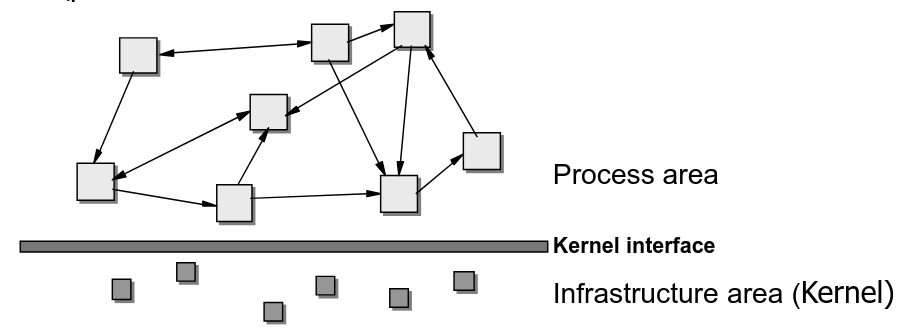
\includegraphics[scale=0.3]{kernelarea.png}
\end{center}

\subsection{Process area}
In more details, the process area is divided like this:
\begin{center}
	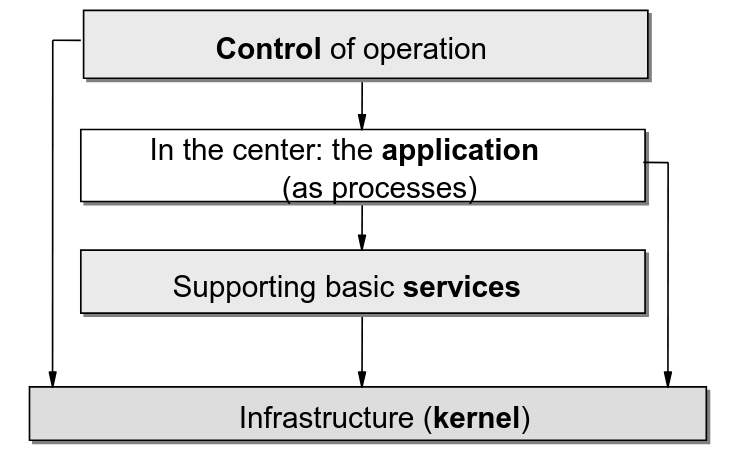
\includegraphics[scale=0.3]{processarea.png}
\end{center}
\subsubsection{Services}
In particular, services deal with \textbf{resources} needed by applications, since handling them directly is very tedious.
\begin{center}
	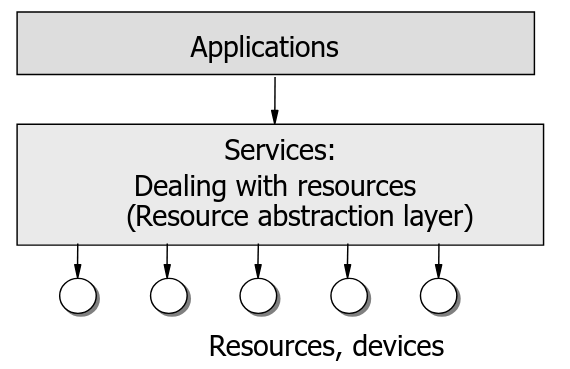
\includegraphics[scale=0.3]{services.png}
\end{center}
Therefore, we need to make a distinction between resources:
\begin{itemize}
	\item \textbf{Logical}: resources for made organizational reasons  by real ones (e.g. files)
	\item \textbf{Physical}: real existent (e.g. mouse, keyboard)
\end{itemize}
The main two aspects of dealing with resources are:
\begin{itemize}
	\item \textbf{Management}: in case of competition, deciding who should get the resource and when
	\begin{center}
		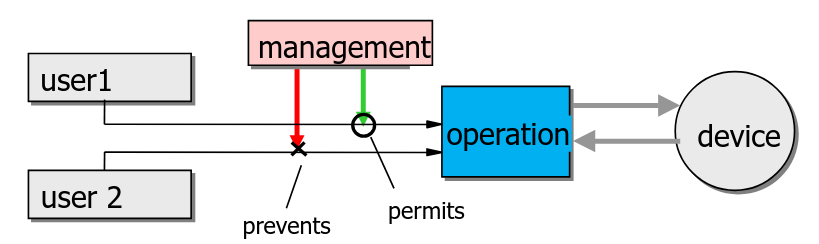
\includegraphics[scale=0.3]{management.png}
	\end{center}
	\item \textbf{Operation}: real usage (e.g. data transport) with \textbf{read} and \textbf{write} operations
	\begin{center}
		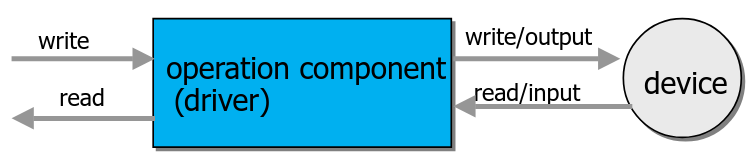
\includegraphics[scale=0.3]{operation.png}
	\end{center}
\end{itemize}
In the end we have both the \textit{management} and the \textit{operation} for the \textit{logical} resources and for the \textit{real} ones.

\subsubsection{Control}
We distinguish two interfaces:
\begin{itemize}
	\item \textbf{Control} interface: handles the interactions between the user and the machine (OS commands and UI)
	\item \textbf{Procedural} interface: has the possibility to make complex requests to the OS, also with programming language notation
\end{itemize}

\subsubsection{Overview}
\begin{center}
	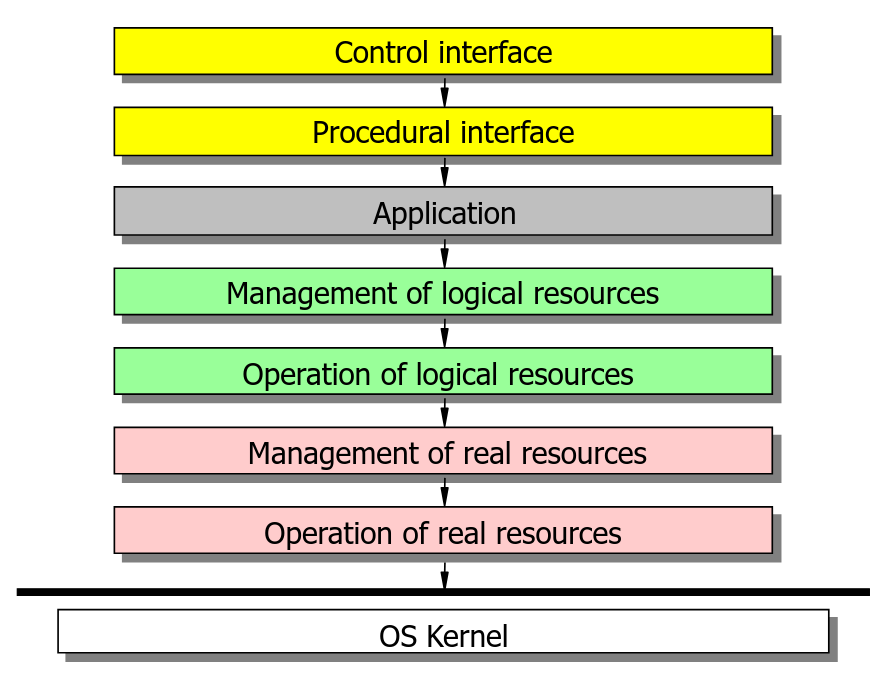
\includegraphics[scale=0.4]{overview.png}
\end{center}

\begin{note}
	Each layer may be \textbf{partitioned} and upward calls are allowed as long as there are no cycles.
\end{note}

\subsection{Kernel area}
In details, the kernel area is divided like this:
\begin{center}
	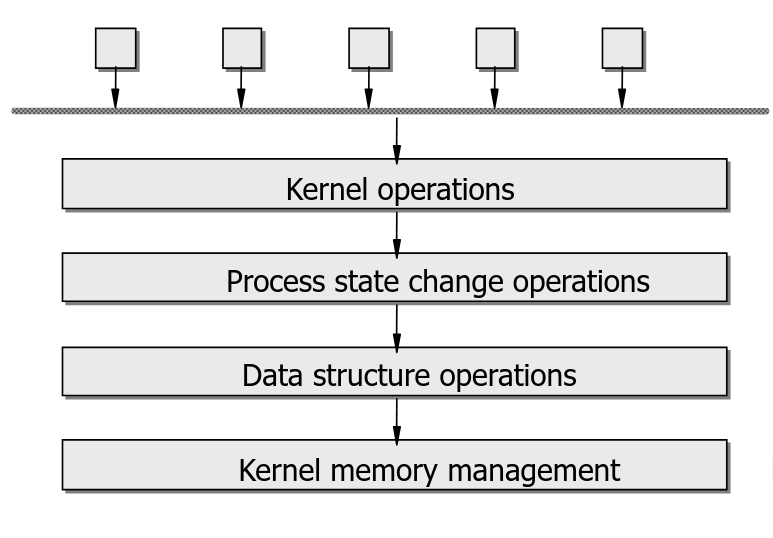
\includegraphics[scale=0.3]{kernelareaover.png}
\end{center}
There are two ways of realizing a kernel:
\begin{itemize}
	\item \textbf{Scattered} across programs: kernel operations resides in different program address spaces
	\item \textbf{Compact}: there is the kernel address space which contains its own procedures
\end{itemize}

\subsubsection{Size}
Depending on what functionalities you add in the kernel, you may end up with different kernel sizes. The bare minimum is the one described above (process management and communication) and it's called \textbf{microkernel}.

\subsubsection{Monolithical}
Another approach is the \textbf{monolithical system}, where there is no strict separation between applications and OS. It's appropriate for small OS.
\begin{center}
	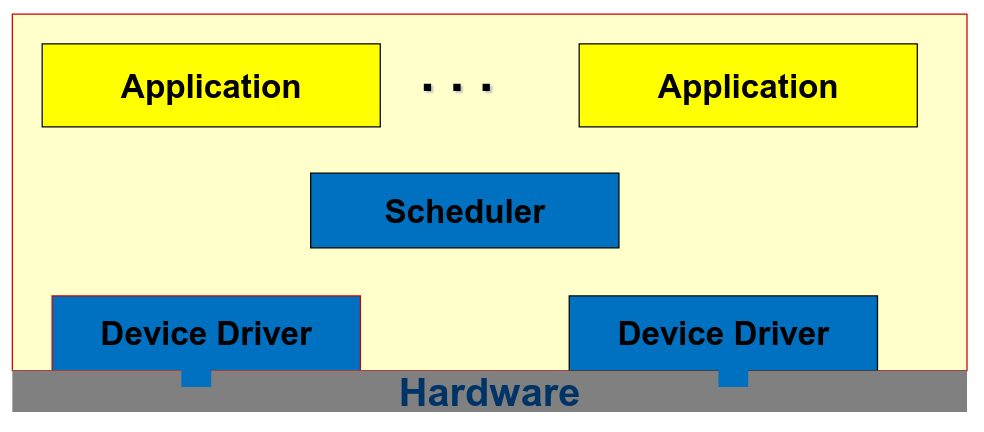
\includegraphics[scale=0.3]{monolit.png}
\end{center}
On the other hand, \textbf{monolithical OS-kernels} have a separation between applications and OS for \textbf{protection} reasons but no separations among OS components.
\begin{center}
	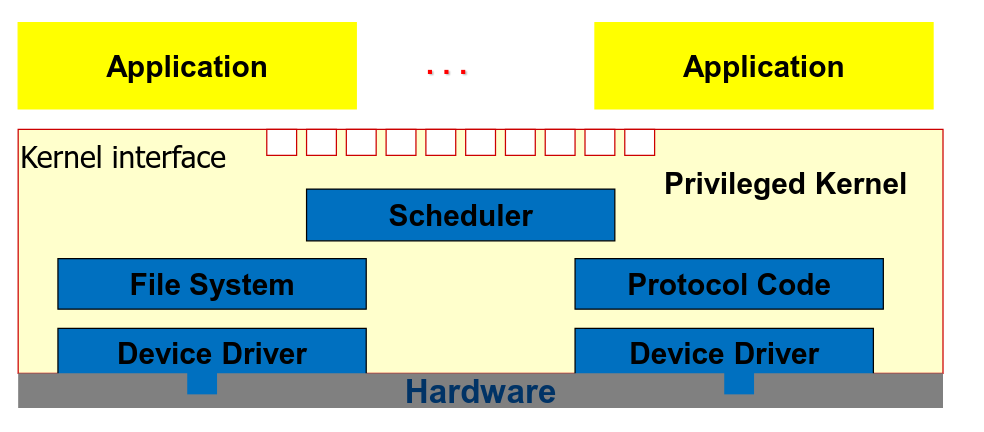
\includegraphics[scale=0.3]{monoker.png}
\end{center}

\subsubsection{Microkernel}
As stated before, a microkernel contains only process management (initializing and dispatching) and Inter Process Communication.
\begin{center}
	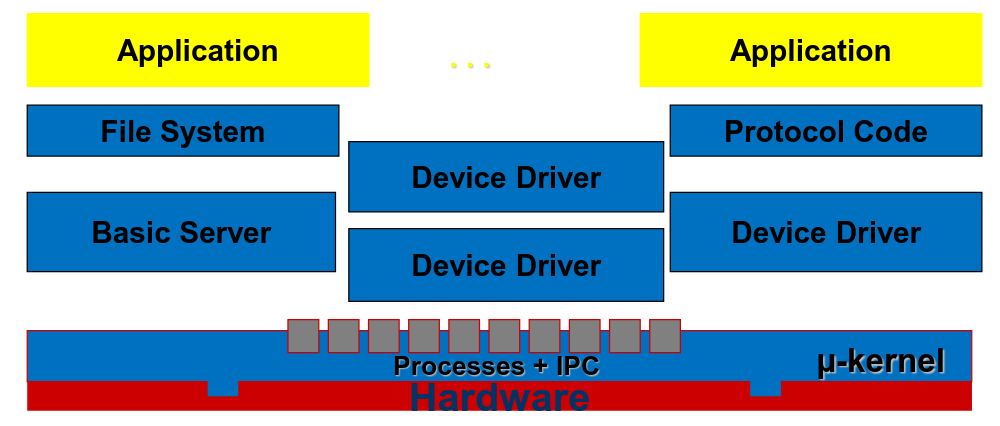
\includegraphics[scale=0.3]{microker.png}
\end{center}
The \textbf{advantages} are:
\begin{itemize}
	\item Supports \textbf{modular} structure
	\item Since the services are outside of the kernel, there is more \textbf{stability} and \textbf{security} because it will not be affected by faulty services. Furthermore it improves \textbf{flexibility} and \textbf{extendibility} since services can be removed and added arbitrarily.
	\item The safety-critical part (kernel) is \textbf{small} and easily verifiable
	\item Usually only the kernel needs to run in \textbf{privileged} mode
	\item It allows the coexistence of several \textbf{interfaces} 
\end{itemize}
The main \textbf{disadvantage} is that there are \textbf{performance} issues since interplay of components outside the kernel need more IPC and therefore more kernel calls.

\subsection{Design principles}
The basic idea is KISS: Keep It Simple and Stupid.
\subsubsection{Modularity}
The system is decomposed in a set of modules so that:
\begin{itemize}
	\item the \textbf{interaction} (information and control flow) within the module is high
	\item the \textbf{interaction} between modules is low
	\item the \textbf{interfaces} between them are simple
	\item the modules are small and easily understandable
\end{itemize}

\subsubsection{Hierarchization}
Homogeneous elements are grouped together in a tree structure to guarantee \textbf{scalability} and mastering complexity.

\subsubsection{Layering}
System functionalities should be divided into layers, with the simpler one at the bottom. Each new layer represents an abstraction of the previous ones and provides an interface for the upper layers.
\begin{example}
	An example of layering is the Internet protocol stack.
\end{example}

\subsubsection{End to end}
A function of service should be carried out within a general layer only if it is \textbf{needed} by all clients of that layer and if it can be completely \textbf{implemented} in that layer.\\
In the OS context this means a \textbf{stable}, \textbf{universal} programming interface should be provided. Support should be placed in the upper layer.
\paragraph{Application neutrality} The OS should be application neutral, meaning that lower layers may provide mechanisms that can be parameterized in higher layers to suit specific application requirements (e.g. scheduling, paging).
\paragraph{Orthogonality} Function and concepts should be independent. Each component should be orthogonal: freedom of combination.
\paragraph{SPOT} Single Point of Truth is a rule to avoid inconsistencies by avoiding repetitions in code (only one implementation) and in data (only one representation).